\documentclass[11pt,a4paper]{article}
\usepackage[margin=2.3cm]{geometry}
\usepackage[T1]{fontenc}
\usepackage{lmodern}
\usepackage{microtype}
\usepackage{booktabs}
\usepackage{tabularx}
\usepackage{enumitem}
\usepackage{xcolor}
\usepackage{listings}
\usepackage{tikz}
\usetikzlibrary{arrows.meta,positioning,fit}
\usepackage{amsmath,amssymb}
\usepackage{graphicx}
\usepackage[hidelinks]{hyperref}

\definecolor{accent}{HTML}{1F5FAD}
\definecolor{codebg}{HTML}{F4F6F8}
\definecolor{warn}{HTML}{B3541E}
\hypersetup{colorlinks=true,linkcolor=accent,urlcolor=accent}
\lstset{basicstyle=\ttfamily\small,backgroundcolor=\color{codebg},frame=single,rulecolor=\color{codebg},
  columns=fullflexible,breaklines=true,xleftmargin=4pt,xrightmargin=4pt,aboveskip=6pt,belowskip=6pt}
\newcommand{\code}[1]{\texttt{\small #1}}
\newcommand{\note}[1]{\par\smallskip\noindent\textcolor{warn}{\textbf{Note.}} #1\par\smallskip}
\setlist{itemsep=2pt,topsep=4pt}

\title{\textbf{Adaptive Adversarial Training (AAT)}\\[4pt]
\large Setup, execution and monitoring guide for the Kaggle rebuild}
\author{Matoke Brian\\\small repository \href{https://github.com/mattobryan/AAT}{\code{github.com/mattobryan/AAT}}, branch \code{matt/funny-planck-3j7md5}}
\date{\today}

\begin{document}
\maketitle
\tableofcontents
\bigskip

\section{Purpose and research question}

This repository rebuilds the MSc thesis \emph{Adaptive Adversarial Training: A Curriculum-Based
Approach to Robustness} (University of Szeged, 2025) so that it runs end to end on free cloud hardware
and can be inspected by others, for example as part of PhD applications. We follow the standard
research method:
\begin{enumerate}
  \item \textbf{Reproduce the baseline} (RAMP, Jiang \& Singh, NeurIPS 2024) with the authors' official
        code until our numbers match the published ones. This gives us RAMP's weights.
  \item \textbf{Lock the baseline}: the reproduced numbers and checkpoints are fixed and stored on the
        Hugging Face Hub.
  \item \textbf{Build AAT on that baseline} and compare it with RAMP under the same starting model,
        training budget and evaluation.
\end{enumerate}

\paragraph{Research question.} Does feedback-driven scheduling of the perturbation budget $\epsilon$
(per class) and of the attacked $\ell_p$ norm improve \emph{union robustness} over
$\{\ell_1,\ell_2,\ell_\infty\}$, and robustness to threats not seen in training, compared with
fixed-schedule multi-norm adversarial training (RAMP, E-AT, MAX)? All evaluation uses AutoAttack at
fixed standard budgets.

\begin{table}[h]
\centering\small
\begin{tabularx}{\linewidth}{@{}lXX@{}}
\toprule
 & Hypothesis & Test \\
\midrule
H1 & Full AAT beats fixed-schedule multi-norm AT on union robustness & \code{aat\_full} vs RAMP, E-AT, MAX; gain $>2\times$ seed std, clean drop $\le 1$\,pp \\
H2 & Class-feedback $\epsilon$ narrows the class robustness gap & worst-class union $\uparrow$, class std $\downarrow$ \\
H3 & Adaptive norm sampling beats cyclic sampling & \code{v2b\_adaptive} vs \code{v2a\_cyclic} \\
H4 & AAT generalises better to unseen threats & larger-$\epsilon$ grid; $\ell_2$ held out of training \\
\bottomrule
\end{tabularx}
\end{table}

\section{System overview}

Nothing needs to run on your laptop. Training runs on Kaggle's servers, checkpoints and logs go to a
private Hugging Face repository, and a scheduled Claude routine reads that repository and sends status
reports to the Claude app on your phone or tablet.

\begin{center}
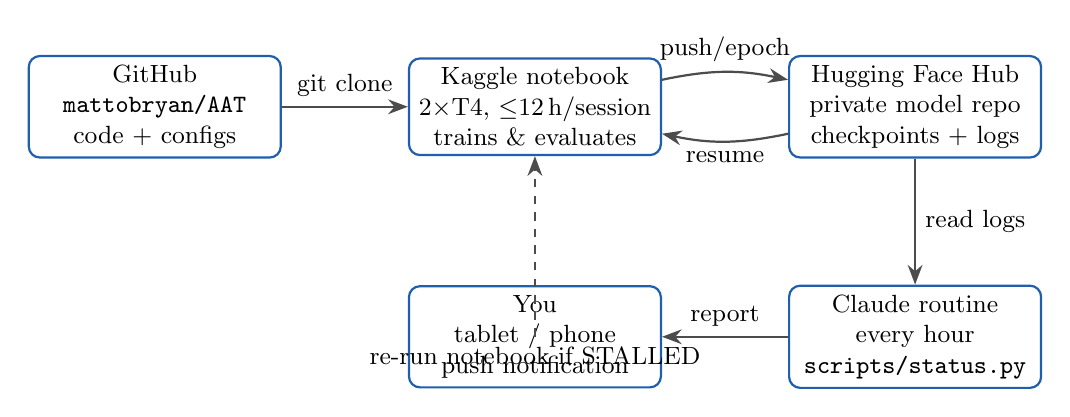
\begin{tikzpicture}[node distance=1.1cm and 1.6cm, font=\small,
  box/.style={draw=accent, rounded corners, thick, align=center, minimum width=3.2cm, minimum height=1.1cm, fill=white},
  arr/.style={-{Stealth[length=2.5mm]}, thick, draw=black!70}]
  \node[box] (gh) {GitHub\\\code{mattobryan/AAT}\\code + configs};
  \node[box, right=of gh] (kg) {Kaggle notebook\\2$\times$T4, $\le$12\,h/session\\trains \& evaluates};
  \node[box, right=of kg] (hf) {Hugging Face Hub\\private model repo\\checkpoints + logs};
  \node[box, below=1.6cm of hf] (rt) {Claude routine\\every hour\\\code{scripts/status.py}};
  \node[box, left=of rt] (tb) {You\\tablet / phone\\push notification};
  \draw[arr] (gh) -- node[above]{git clone} (kg);
  \draw[arr] (kg) to[bend left=12] node[above]{push/epoch} (hf);
  \draw[arr] (hf) to[bend left=12] node[below]{resume} (kg);
  \draw[arr] (hf) -- node[right]{read logs} (rt);
  \draw[arr] (rt) -- node[above]{report} (tb);
  \draw[arr, dashed] (tb) -| node[near start, below]{re-run notebook if STALLED} (kg);
\end{tikzpicture}
\end{center}

\section{Repository layout}

\begin{table}[h]
\centering\small
\begin{tabularx}{\linewidth}{@{}lX@{}}
\toprule
Path & Content \\
\midrule
\code{aat/models.py} & PreActResNet-18 (ReLU), and the RAMP/E-AT softplus variant that loads the official \code{pretr\_*.pth} weights (verified: identical logits, max diff $5\times10^{-7}$) \\
\code{aat/attacks.py} & PGD under $\ell_\infty,\ell_2,\ell_1$ with per-sample budgets (training only) \\
\code{aat/schedulers.py} & adaptive $\epsilon$ (static, linear, norm/class feedback, per-sample) and norm schedulers \\
\code{aat/losses.py} & max / mean / hybrid multi-norm losses, RAMP KL logit pairing \\
\code{aat/train.py} & feedback $\rightarrow$ adapt $\rightarrow$ adversarial-training loop, resume + HF sync \\
\code{aat/evaluate.py} & AutoAttack (APGD-CE + APGD-T, official RAMP settings), union, per-class, unseen grid \\
\code{aat/hub.py} & Hugging Face push/pull, history squashing, never crashes training \\
\code{baselines/} & published target numbers; resume/HF patch for the official \code{RAMP.py} \\
\code{scripts/} & \code{ramp\_official.sh}, \code{compare\_targets.py}, \code{status.py}, \code{aggregate.py}, \code{run\_queue.sh} \\
\code{configs/} & one YAML per method (baselines and AAT ablations) \\
\code{notebooks/} & \code{ramp\_baseline\_kaggle.ipynb} (step 1), \code{aat\_kaggle.ipynb} (step 2) \\
\code{docs/} & thesis audit, RAMP reproduction notes, this guide \\
\bottomrule
\end{tabularx}
\end{table}

\section{Step 1: the RAMP baseline}

\subsection{Targets}
Published values (\%), AutoAttack, first 1{,}000 CIFAR-10 test points.

\begin{table}[h]
\centering\small
\resizebox{\linewidth}{!}{\begin{tabular}{@{}lccccc l@{}}
\toprule
Setting & Clean & $\ell_\infty$ & $\ell_2$ & $\ell_1$ & Union & Role \\
\midrule
RAMP from scratch, 80 ep, $\lambda{=}5$, GP (paper Tab.~3) & 81.2 & 46.0 & 65.8 & 48.3 & 44.6 & \textbf{thesis baseline} \\
Thesis Table 7.1 (5 runs)                          & 81.3 & 45.96 & 65.74 & 48.42 & 44.5 & to match \\
RAMP fine-tune 3 ep, $\lambda{=}1.5$ (paper Tab.~24) & 81.1 & 45.4 & 66.1 & 47.2 & 43.1 & cross-check \\
\code{pretr\_Linf} (fine-tuning start)             & 83.7 & 48.1 & 59.8 & 7.7 & $\approx$7 & sanity \\
\bottomrule
\end{tabular}}
\end{table}

\subsection{What is run}
The \textbf{official code} (\code{uiuc-focal-lab/RAMP}, pinned commit \code{be4971f}) is cloned during
setup. Two changes are applied, both reviewable:
\begin{itemize}
  \item \code{import copy} added to \code{utils.py} (the \code{--gp} path otherwise raises \code{NameError});
  \item \code{baselines/ramp\_resume\_hub.patch} ($\approx$90 lines): \code{--resume} restores both models,
        both optimisers and all RNG states; \code{--time\_budget\_h} exits cleanly after the last epoch that
        fits; \code{--hf\_repo} pushes the resume checkpoint, logs and \code{ep\_*.pth} after every epoch.
        The training algorithm is untouched.
\end{itemize}
Our evaluator then scores every checkpoint with AutoAttack \code{standard} settings restricted to
APGD-CE and APGD-T (for $\ell_1$: 5 restarts, 5 target classes). Seed 0 is also scored by the official
\code{eval.py} on the same points, as a check of our evaluator.

\subsection{Acceptance}
Per metric: \textbf{OK} if $|\Delta|\le1$\,pp from the target, \textbf{CLOSE} if $\le2$\,pp (report with
an explanation), otherwise \textbf{OFF} (investigate before building AAT).

\section{One-time setup}

\subsection{Hugging Face}
\begin{enumerate}
  \item Create a free account at \url{https://huggingface.co}.
  \item Settings $\rightarrow$ Access Tokens $\rightarrow$ \emph{New token}, type \textbf{Write}. Copy it.
  \item Choose a repository name, e.g.\ \code{<hf-username>/aat-checkpoints}. You do not need to create
        it: the first push creates it as \textbf{private}.
\end{enumerate}

\subsection{Kaggle}
\begin{enumerate}
  \item Verify your phone number (Settings), which is required for GPUs and internet access.
  \item Create a notebook via \emph{File $\rightarrow$ Import notebook}, choose GitHub, repository
        \code{mattobryan/AAT}, and select the file \code{notebooks/ramp\_baseline\_kaggle.ipynb}.
        You can also upload the \code{.ipynb} from a local clone.
  \item \emph{Add-ons $\rightarrow$ Secrets $\rightarrow$ Add secret}: label \code{HF\_TOKEN}, value = the
        write token. Tick it for this notebook.
  \item Session options: Accelerator \textbf{GPU T4 $\times$2}, Internet \textbf{on}, Persistence
        \emph{Files only}.
  \item In the first code cell, set \code{HF\_REPO} to your repository name.
\end{enumerate}

\subsection{Monitoring (Claude routine)}
The cloud environment of the Claude session that runs the routine needs two environment variables.
Add them in the environment settings (session title bar $\rightarrow$ cloud environment $\rightarrow$
Edit), \emph{never} in a chat message:
\begin{itemize}
  \item \code{HF\_TOKEN}: a Hugging Face token. A \textbf{read} token is enough here, so create a
        second, read-only token.
  \item \code{HF\_REPO}: the same repository name as on Kaggle.
\end{itemize}
Until both are set, every report reads ``monitor not configured''.

\section{Running}

\subsection{A session}
\begin{enumerate}
  \item Open the notebook on Kaggle and click \textbf{Save Version $\rightarrow$ Save \& Run All (Commit)}.
        The run continues on Kaggle's servers after you close the browser, up to 12 hours.
  \item Setup cell: clones the repository and the official RAMP code, applies the patch, installs
        dependencies and downloads CIFAR-10 ($\approx$3 min).
  \item Sanity cell: evaluates \code{pretr\_Linf}. Expect $\approx$83.7 / 48.1 / 59.8 / 7.7 / union ≈ 7.
  \item Stage A: RAMP from scratch, seed~0 on GPU~0 and seed~1 on GPU~1. Each run stops at 11\,h and
        pushes its checkpoint.
\end{enumerate}

\subsection{Resuming}
When a report says \textbf{STALLED}, or the Kaggle version shows \emph{complete} while a run is not
\textbf{DONE}, run the notebook again (same button). It pulls \code{resume.pth} from the Hub and
continues from the last finished epoch. Finished runs are recognised and skipped. Repeat until both
seeds are \textbf{DONE}, then change the seed lists to \code{"2" "3"} and later \code{"4"}.

\subsection{Evaluating and comparing}
After the seeds finish, the evaluation cell scores them and prints the comparison:
\begin{lstlisting}
bash scripts/ramp_official.sh eval ramp_scratch "0 1" 0
python scripts/compare_targets.py --runs runs_official --table thesis_table7_1 --map ramp_scratch_official=ramp
python scripts/compare_targets.py --runs runs_official --table scratch_table3  --map ramp_scratch_official=ramp_l5
\end{lstlisting}
Stage B (the fine-tuning cross-check, $\approx$1 GPU-hour per seed) can run on leftover session time.

\section{Monitoring and reports}

The routine runs every hourutes in a fresh cloud session. It checks out the branch, runs
\code{python scripts/status.py}, and sends a short report to the Claude app. Example:
\begin{lstlisting}
AAT status 2026-09-26 14:30 UTC (user/aat-checkpoints)
- ramp_scratch_l5_s0: running | epoch 37/80 | 15 min/epoch | last push 6 min ago | ETA 10.8 GPU-h
    Linf 44.0% L2 63.5% L1 46.0% clean 78.5% union 42.5%
- ramp_scratch_l5_s1: STALLED - re-run the notebook | epoch 41/80 | ...
\end{lstlisting}

\begin{table}[h]
\centering\small
\begin{tabularx}{\linewidth}{@{}lX@{}}
\toprule
State & Meaning and action \\
\midrule
\code{running} & a push arrived within $2\times$ the mean epoch time $+$ 20 min. Nothing to do. \\
\code{STALLED} & no push for longer. Usually the 11\,h budget or the 12\,h limit ended the session: re-run the notebook. If it happens within minutes of starting, open the Kaggle log (likely a setup error). \\
\code{DONE} & all epochs finished. Run the evaluation cell. \\
\code{monitor not configured} & \code{HF\_TOKEN} / \code{HF\_REPO} are missing from the routine's environment. \\
\bottomrule
\end{tabularx}
\end{table}
The in-training numbers in the report come from 200 points and 100-step APGD. They are for tracking
only. Reported results come exclusively from the final AutoAttack evaluation.

\section{Step 2: AAT experiments}

Once the baseline is locked, AAT runs through \code{aat/train.py} with the same HF sync and time
budget. The primary comparison starts AAT from the same model as RAMP, with the same budget and the
same evaluation, so any difference is due to adaptive scheduling. Continuing from the RAMP weights is
optional and needs a control in which RAMP also continues for the same number of epochs.

\begin{table}[h]
\centering\small
\begin{tabularx}{\linewidth}{@{}llX@{}}
\toprule
Config & Thesis name & What changes \\
\midrule
\code{v3a\_max} & 3A & all three norms, fixed $\epsilon$, per-sample worst case \\
\code{v1a\_linear} & 1A & $+$ global linear $\epsilon$ ramp \\
\code{v1b\_sample} & 1B & $+$ per-sample, class-aware $\epsilon$ (gradient norm + class robustness) \\
\code{v2a\_cyclic} / \code{v2b\_adaptive} & 2A / 2B & one norm per batch: round-robin vs Boltzmann on feedback \\
\code{v3b\_classeps} & 3B & class-feedback $\epsilon$ controller, Eq.~(4.19) \\
\code{aat\_full} & full AAT & $+$ adaptive norm weights, hybrid loss, KL pairing \\
\code{aat\_full\_no\_l2} & unseen norm & full AAT trained without $\ell_2$ \\
\bottomrule
\end{tabularx}
\end{table}
Before AAT results are trusted, \code{configs/ramp.yaml} (our reimplementation) must reproduce the
locked official RAMP numbers. That check comes first in step 2.

\section{Evaluation protocol}
\begin{itemize}
  \item Fixed budgets only: $\ell_\infty = 8/255$, $\ell_2 = 0.5$, $\ell_1 = 12$. Adaptive $\epsilon$ is never used at test time.
  \item AutoAttack APGD-CE + APGD-T, first 1{,}000 test points (the protocol of the RAMP fine-tuning
        table, confirmed by the 83.7\,\% clean accuracy of \code{pretr\_Linf}).
  \item Union = per-sample AND over the three norms (not the minimum of the three accuracies).
  \item Unseen threats: $\ell_\infty\in\{4,12,16\}/255$, $\ell_2\in\{0.25,1,1.5\}$, $\ell_1\in\{6,18,24\}$, and $\ell_2$ for runs trained without it.
  \item The test set is never used for adaptation or model selection. The last checkpoint is always used.
\end{itemize}

\section{Budget and schedule}
Kaggle gives about 30 GPU-hours per week and at most 12 hours per session. The figures below are
estimates: the first logged epoch time replaces them.

\begin{table}[h]
\centering\small
\begin{tabular}{@{}lrr@{}}
\toprule
Job & est.\ T4 time & sessions \\
\midrule
Setup + \code{pretr\_Linf} sanity & 15 min & -- \\
RAMP from scratch, 1 seed (80 ep, GP, fp32) & 15--25 h & 2--3 \\
two seeds in parallel (2$\times$T4) & same wall time & 2--3 \\
RAMP fine-tune cross-check, 5 seeds & $\approx$5 GPU-h & 1 \\
AutoAttack eval, 1{,}000 points, per model & 10--30 min & -- \\
\bottomrule
\end{tabular}
\end{table}
\note{Five from-scratch seeds cost more than one week's quota. Plan: seeds 0--1 in week 1, together with
the fine-tuning cross-check; seeds 2--4 in week 2, in parallel with the first AAT runs. Two seeds
already give a mean and spread to compare with the thesis Table 7.1.}

\section{Troubleshooting}
\begin{table}[h]
\centering\small
\begin{tabularx}{\linewidth}{@{}lX@{}}
\toprule
Symptom & Fix \\
\midrule
\code{[hub] WARNING push failed} & transient network or rate limit; the next epoch pushes again. If it repeats, check that the token has \emph{write} scope and that \code{HF\_REPO} is spelled correctly. \\
\code{nothing to pull} on the first run & expected: no checkpoint exists yet. \\
Setup fails on \code{git apply} & the patch is already applied (the setup script skips it) or the pinned commit changed; re-run setup in a fresh session. \\
CUDA out of memory & another run is using the same GPU: check \code{CUDA\_VISIBLE\_DEVICES} in the cell (0 and 1). \\
Sanity numbers far from 83.7 clean / 48.1 $\ell_\infty$ & evaluation or data problem: stop and investigate before training. \\
Result OFF by $>2$\,pp & compare the seed-0 official eval log with ours; check the epoch count and $\lambda$ in \code{log\_train.txt}. \\
\bottomrule
\end{tabularx}
\end{table}

\section{Checklist}
\begin{enumerate}[label=$\square$]
  \item HF write token created; Kaggle secret \code{HF\_TOKEN} added and enabled for the notebook
  \item \code{HF\_REPO} set in the notebook's first cell
  \item Read-only HF token and \code{HF\_REPO} added to the Claude environment (for reports)
  \item Session 1: Save \& Run All; the sanity numbers match
  \item Re-run on every \textbf{STALLED} report until seeds 0--1 are \textbf{DONE}
  \item Evaluate, then run \code{compare\_targets.py}: all OK or CLOSE $\Rightarrow$ baseline locked
  \item Step 2: \code{configs/ramp.yaml} reproduces the locked baseline, then the AAT runs start
\end{enumerate}

\appendix
\section{Command reference}
\begin{lstlisting}
# official baseline (inside the Kaggle notebook or any GPU shell)
export HF_REPO=<hf-username>/aat-checkpoints  HF_TOKEN=...   # token via Kaggle secret on Kaggle
bash scripts/ramp_official.sh setup
bash scripts/ramp_official.sh pretr 0
bash scripts/ramp_official.sh train ramp_scratch "0" 0        # resumes automatically
bash scripts/ramp_official.sh eval  ramp_scratch "0 1" 0
bash scripts/ramp_official.sh train ramp "0 1 2 3 4" 0        # fine-tuning cross-check

# AAT (step 2)
python -m aat.train --config configs/aat_full.yaml --set seed=0
python -m aat.evaluate --run runs/aat_full_s0
python scripts/aggregate.py --runs runs

# status from anywhere
python scripts/status.py
\end{lstlisting}

\end{document}
